\documentclass[border=4pt]{standalone}
\usepackage[T1]{fontenc}
\usepackage{lmodern}
\usepackage{tikz}
\usetikzlibrary{arrows.meta,positioning}
\begin{document}
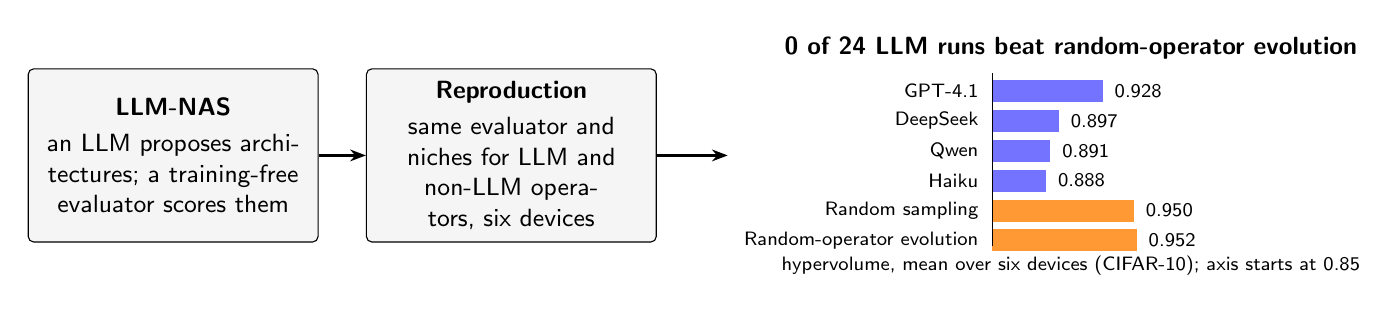
\begin{tikzpicture}[font=\sffamily\small,>={Stealth[length=2mm]},
  box/.style={draw,rounded corners=2pt,align=center,fill=gray!8,inner sep=4pt,text width=3.4cm,minimum height=2.2cm}]
\node[box] (a) {\textbf{LLM-NAS}\\[2pt]an LLM proposes architectures; a training-free evaluator scores them};
\node[box,right=6mm of a] (b) {\textbf{Reproduction}\\[2pt]same evaluator and niches for LLM and non-LLM operators, six devices};
\draw[->,thick] (a)--(b);
\begin{scope}[shift={(10.4,-1.1)}]
  \def\s{18}
  \foreach \lab/\v/\c [count=\i] in {GPT-4.1/0.928/blue!55, DeepSeek/0.897/blue!55, Qwen/0.891/blue!55, Haiku/0.888/blue!55,
      {Random sampling}/0.950/orange!80, {Random-operator evolution}/0.952/orange!80} {
    \pgfmathsetmacro{\w}{(\v-0.85)*\s}
    \pgfmathsetmacro{\y}{2.3-0.38*\i}
    \fill[\c] (0,\y-0.14) rectangle (\w,\y+0.14);
    \node[anchor=east,font=\sffamily\scriptsize] at (-0.05,\y) {\lab};
    \node[anchor=west,font=\sffamily\scriptsize] at (\w+0.03,\y) {\v};
  }
  \draw (0,-0.05)--(0,2.15);
  \node[font=\sffamily\scriptsize,anchor=north] at (1.0,-0.05) {hypervolume, mean over six devices (CIFAR-10); axis starts at 0.85};
  \node[font=\sffamily\small\bfseries,anchor=south,align=center] at (1.0,2.2) {0 of 24 LLM runs beat random-operator evolution};
\end{scope}
\draw[->,thick] (b.east)--++(0.9,0);
\end{tikzpicture}
\end{document}
